% Figure 4.1. Full design domain and its left-half symmetry-reduced domain.
% Build in WSL: latex + dvips -E for EPS, pdflatex for PDF, pdftocairo for PNG.
\documentclass[tikz,border=3pt]{standalone}
\usepackage{amsmath}
\usepackage{tikz}
\usetikzlibrary{arrows.meta}

\begin{document}
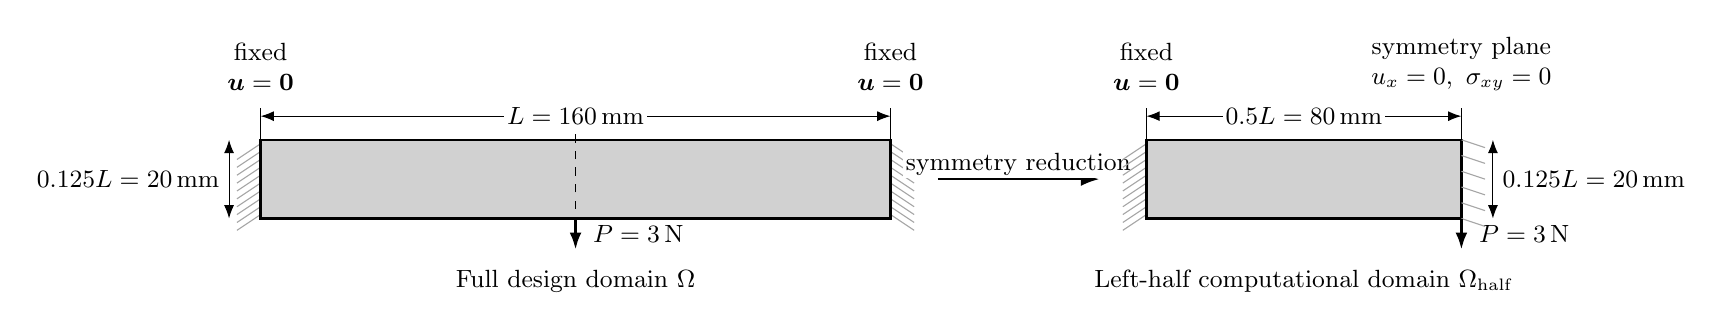
\begin{tikzpicture}[x=0.05cm,y=0.05cm,>=Latex]
  \def\L{160}
  \def\H{20}
  \def\Lhalf{80}
  \def\Xhalf{225}  % 左半域左端横坐标, 与完整域右端留出 65 单位间隙

  % ================= 完整设计域 (左) =================
  \draw[thick,fill=black!18] (0,0) rectangle (\L,\H);
  % 左右固支端阴影线
  \foreach \y in {0,2,...,18} {
    \draw[gray!70] (-6,\y-3) -- (0,\y+1);
    \draw[gray!70] (\L+6,\y-3) -- (\L,\y+1);
  }
  \draw[thick] (0,0) -- (0,\H);
  \draw[thick] (\L,0) -- (\L,\H);
  % 对称轴 (竖直虚线)
  \draw[dashed] (0.5*\L,-6) -- (0.5*\L,\H+2);

  % 尺寸标注
  \draw[thin] (0,\H) -- (0,\H+8);
  \draw[thin] (\L,\H) -- (\L,\H+8);
  \draw[<->,thin] (0,\H+6) -- (\L,\H+6)
    node[midway,fill=white,inner sep=1pt,font=\small] {$L=160\,\mathrm{mm}$};
  % 高度标注放在左端外侧, 避免占用两域之间的间隙 (留给对称降维箭头)
  \draw[<->,thin] (-8,0) -- (-8,\H)
    node[midway,left,font=\small] {$0.125L=20\,\mathrm{mm}$};

  % 边界条件标注
  \node[font=\small,align=center,anchor=south] at (0,\H+10)
    {fixed\\$\boldsymbol{u}=\boldsymbol{0}$};
  \node[font=\small,align=center,anchor=south] at (\L,\H+10)
    {fixed\\$\boldsymbol{u}=\boldsymbol{0}$};

  % 中点载荷
  \draw[very thick,-{Latex[length=2.2mm,width=1.5mm]}] (0.5*\L,0) -- (0.5*\L,-8);
  \node[font=\small,anchor=west] at (0.5*\L+2,-4) {$P=3\,\mathrm{N}$};
  \node[font=\small,align=center] at (0.5*\L,-16)
    {Full design domain $\Omega$};

  % ============ 对称降维箭头 (单行标注, 位于两域之间的间隙) ============
  \draw[->,thick] (\L+12,0.5*\H) -- (\Xhalf-12,0.5*\H)
    node[midway,above,font=\small,fill=white,inner sep=1pt] {symmetry reduction};

  % ================= 左半设计域 (右) =================
  \draw[thick,fill=black!18] (\Xhalf,0) rectangle (\Xhalf+\Lhalf,\H);
  % 左端固支阴影线
  \foreach \y in {0,2,...,18} {
    \draw[gray!70] (\Xhalf-6,\y-3) -- (\Xhalf,\y+1);
  }
  \draw[thick] (\Xhalf,0) -- (\Xhalf,\H);
  % 对称面 (右端) 阴影线
  \draw[thick] (\Xhalf+\Lhalf,0) -- (\Xhalf+\Lhalf,\H);
  \foreach \y in {0,4,...,20} {
    \draw[gray!70] (\Xhalf+\Lhalf,\y) -- (\Xhalf+\Lhalf+6,\y-2);
  }

  % 尺寸标注
  \draw[thin] (\Xhalf,\H) -- (\Xhalf,\H+8);
  \draw[thin] (\Xhalf+\Lhalf,\H) -- (\Xhalf+\Lhalf,\H+8);
  \draw[<->,thin] (\Xhalf,\H+6) -- (\Xhalf+\Lhalf,\H+6)
    node[midway,fill=white,inner sep=1pt,font=\small] {$0.5L=80\,\mathrm{mm}$};
  \draw[<->,thin] (\Xhalf+\Lhalf+8,0) -- (\Xhalf+\Lhalf+8,\H)
    node[midway,right,font=\small] {$0.125L=20\,\mathrm{mm}$};

  % 边界条件标注
  \node[font=\small,align=center,anchor=south] at (\Xhalf,\H+10)
    {fixed\\$\boldsymbol{u}=\boldsymbol{0}$};
  \node[font=\small,align=center,anchor=south] at (\Xhalf+\Lhalf,\H+10)
    {symmetry plane\\$u_x=0,\ \sigma_{xy}=0$};

  % 对称面底端载荷
  \draw[very thick,-{Latex[length=2.2mm,width=1.5mm]}] (\Xhalf+\Lhalf,0) -- (\Xhalf+\Lhalf,-8);
  \node[font=\small,anchor=west] at (\Xhalf+\Lhalf+2,-4) {$P=3\,\mathrm{N}$};
  \node[font=\small,align=center] at (\Xhalf+0.5*\Lhalf,-16)
    {Left-half computational domain $\Omega_{\mathrm{half}}$};
\end{tikzpicture}
\end{document}
